\chapter{Background}
\label{cha:background}

In this chapter, we introduce the necessary logical and compiler background concepts required for the understanding of the material presented in this thesis. In Section~\ref{sec:lambda_calc}, we review some of the mathematical background useful for understanding our optimisations. In Section~\ref{sec:background_agda}, we give an introduction to the Agda compiler.

\section{Lambda Calculus}
\label{sec:lambda_calc}

Lambda calculus (or $\lambda$-calculus) is a formal system for representing computational logic in terms of function abstractions and applications using variable binding and substitution. It warrants our understanding because concepts surrounding the Agda programming language and its compilation are inspired by, and can be elegantly explained by, the framework of the lambda calculi. In fact, the namesake of the default Agda GHC backend, MAlonzo, is Alonzo Church, the mathematician who first developed the lambda calculus \citep{fokkinga1987}.

\subsection{Pure $\lambda$-Calculus}

In a pure $\lambda$-calculus, terms are built inductively from only variables, $\lambda$-abstractions and applications, as in Figure~\ref{fig:lambda_calc} \citep{kozen1997}.

\begin{figure}[h]
\begin{align*}
t ::=~& x               & \text{variable}\\
    |~& \lambda x . t   & \text{abstraction}\\
    |~& t~t             & \text{application}
\end{align*}
\caption{Grammar of a pure lambda calculus.}
\label{fig:lambda_calc}
\end{figure}

\subsection{De Bruijn Index Notation}

In order to eliminate the need for named variables in $\lambda$-calculus notation, de Bruijn indexed notation is used to represent bound terms (variables) with natural numbers, as presented by \citet{deBruijn-1972}. In any term, the positive integer $n$ refers to the $n$th surrounding $\lambda$ binder. In other words, the number is an index indicating the number of variable binders (or $\lambda$-abstractions) in scope between itself and the binder for the variable being referenced. The grammar of a de Bruijn-indexed lambda calculus can be seen in Figure~\ref{fig:db_lambda_calc}. See Figure~\ref{fig:db_example} for an illustration where the variable bindings and indices are coloured to indicate matches and the references are shown with arrows.

\begin{figure}[h]

% \begin{equation*}
%   \textcolor{blue}{\lambda x} . (\textcolor{red}{\lambda y} . (\lambda z . \textcolor{red}{y}) \textcolor{red}{y}) \textcolor{blue}{x}
% \end{equation*}
%
% \begin{equation*}
%   \textcolor{blue}{\lambda}\ (\textcolor{red}{\lambda}\ (\lambda\ \textcolor{red}{1})\ \textcolor{red}{0})\ \textcolor{blue}{0}
% \end{equation*}

\centering
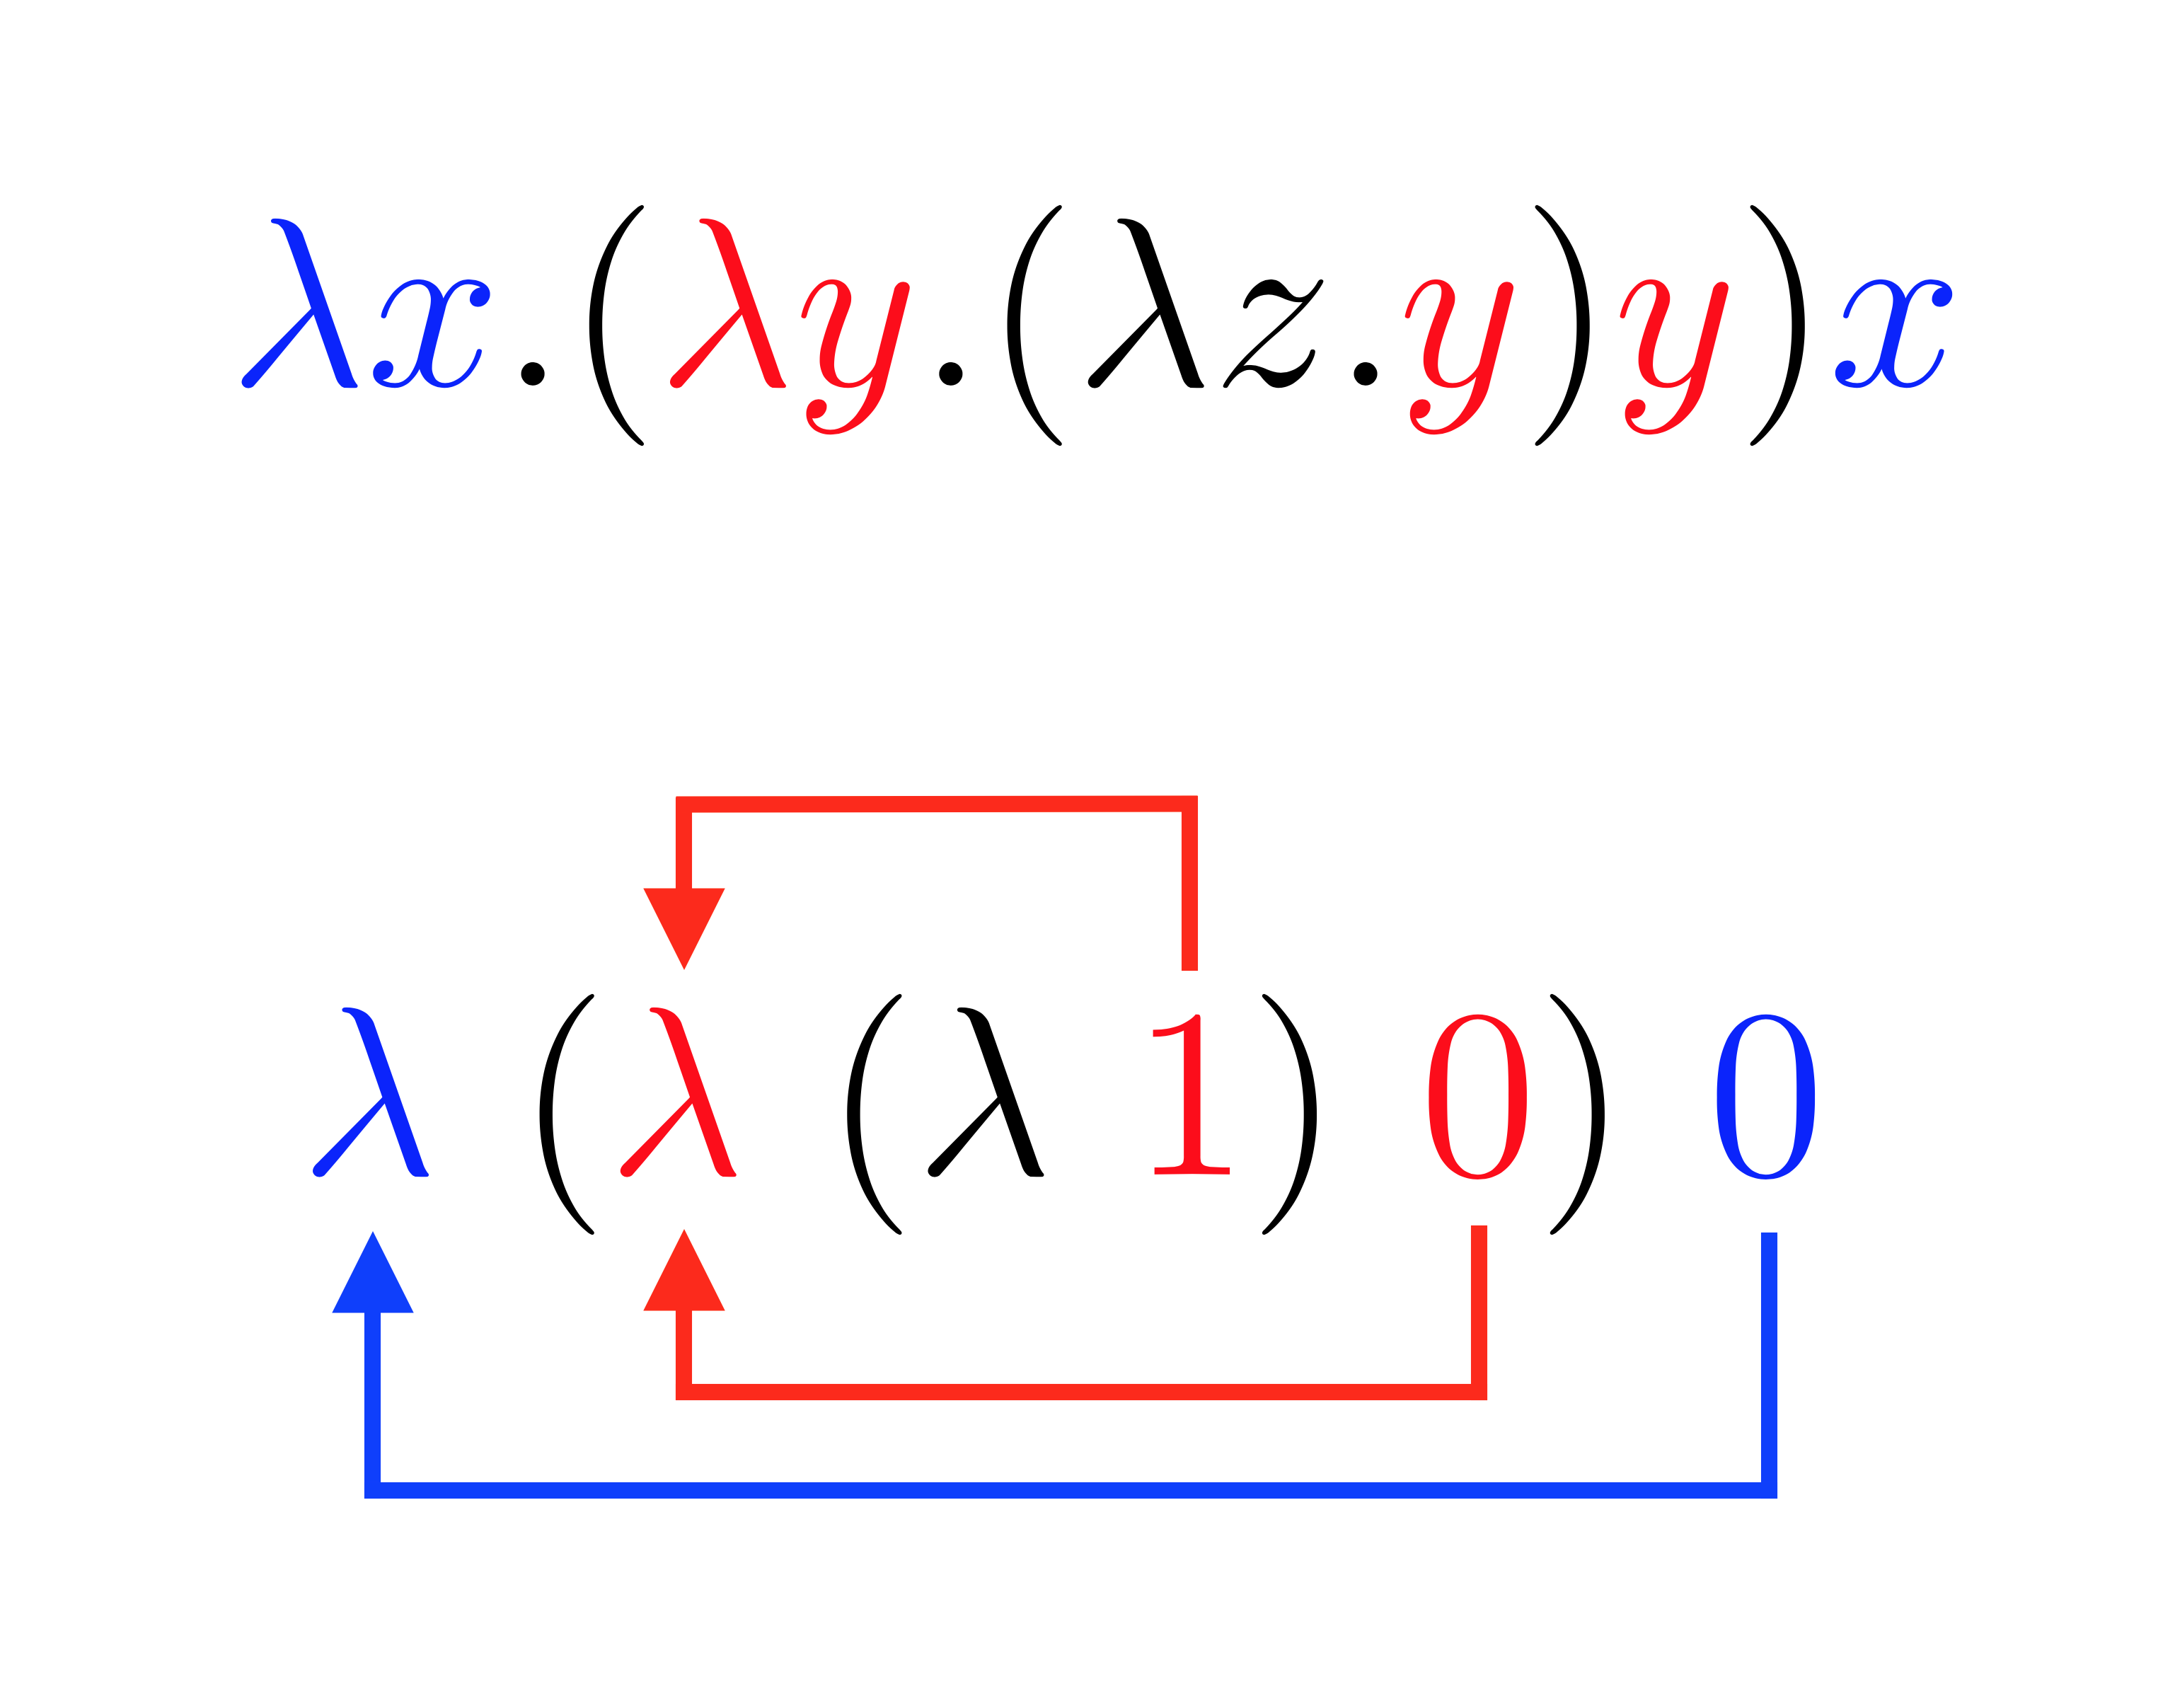
\includegraphics[width=9cm]{Figures/DeBruijnIndex}

\caption{An example of a (circumlocutious) identity function as a de Bruijn indexed $\lambda$-calculus expression.}
\label{fig:db_example}
\end{figure}


\begin{figure}[h]
\begin{align*}
t ::=~& \mathbb{N}      & \text{variable}\\
    |~& \lambda~t       & \text{abstraction}\\
    |~& t~t             & \text{application}
\end{align*}
\caption{Grammar of a de Bruijn indexed lambda calculus.}
\label{fig:db_lambda_calc}
\end{figure}

The internal representation of Agda code in the compiler is based on a de Bruijn indexed $\lambda$-calculus.

\subsection{$\lambda\sigma$-Calculus}

In order to perform the desired optimisations on the abstract syntax tree, we must be able to perform substitutions on terms. Treating the abstract syntax tree structure as a specialised $\lambda$-calculus, we can implement substitution as a function on terms.

Because our terms are built on de Bruijn indexed variables, we use \citet{Abadi-Cardelli-Curien-Levy-1990}'s explicit substitution of a $\lambda\sigma$-calculus as a reference for understanding correct substitution on terms in the context of local variables bound by incrementing indices. The $\lambda\sigma$-calculus is a refinement of the $\lambda$-calculus where substitutions are manipulated explicitly, and substitution application is a term constructor rather than a meta-level notation.

\subsection{Substitution}
\label{sub:lambda_calc_subst}

Take then, for instance, a simple case of the classical application of the $\beta$-rule (See Figure~\ref{eq:beta_rule}). Beta reduction is the process of simplifying an application of a function to the resulting substituted term. However, in order to $\beta$-reduce $(\lambda a)b$, we must not only substitute $b$ into the appropriate occurrences in $a$. As the $\lambda$ binding disappears, we must also decrement all remaining free indices in $a$. This adapted form of the $\beta$-rule can be represented by the infinite substitution shown in Figure~\ref{eq:beta_rule2}) \citep{Abadi-Cardelli-Curien-Levy-1990}.

\begin{figure}[h]
\begin{equation*}
(\lambda x.t)s \to_{\beta} t[x := s]
\end{equation*}
\caption{The classical $\beta$-reduction rule.}
\label{eq:beta_rule}
\end{figure}

\begin{figure}[h]
\begin{equation*}
(\lambda t)s \to_{\beta} t[1 := s, 2 := 1, 3 := 2, ...]
\end{equation*}
\caption{The modified $\beta$-reduction rule for de Bruijn notation.}
\label{eq:beta_rule2}
\end{figure}

However, the substitution in this adapted rule must be evaluated carefully to produce a correct result. Consider if the term $t$ contains another $\lambda$ binding. As the substitution is applied to that nested $\lambda$ term, occurrences of $1$ should not be replaced with $s$, because occurrences of $1$ refer to the nested $\lambda$ term's bound variable. Instead, occurrences of $2$ should be replaced with $s$; likewise, occurrences of $3$ should be replaced by $2$, and so on. We thus ``shift'' the substitution \citep{Abadi-Cardelli-Curien-Levy-1990}.

It is also important when applying substitutions to $\lambda$ terms that we avoid the unintended capture of free variables in our terms being substituted in. Imagine again the nested $\lambda$ term, with occurrences of $2$ being replaced with $s$. Occurrences of $1$ in $s$ must be replaced with $2$, else the nested $\lambda$ binder will capture the index. We this ``lift'' the indices of $s$. These two caveats result in the substitution rule in Figure~\ref{eq:debruijn_sub} \citep{Abadi-Cardelli-Curien-Levy-1990}.

\begin{figure}[h]
\begin{equation*}
(\lambda t)[1 := s, 2 := 1, ...] = \lambda t[2 := s[1 := 2, 2 := 3, ...], 3 := 2, ...]
\end{equation*}
\caption{The substitution rule for de Bruijn indexed lambda terms.}
\label{eq:debruijn_sub}
\end{figure}

Recognising the required index ``shifting'' and ``lifting'' in the Figure~\ref{eq:debruijn_sub} substitution rule should suffice as background for understanding the variable manipulation performed in our optimisation.

\section{Agda}
\label{sec:background_agda}

\subsection{Compiler}

The Agda programming language's first and most-used backend is MAlonzo, or more generically, the GHC backend \citep{benke2007}. Given an Adga module containing a \AgdaFunction{main} function\footnote{An Agda module without a main file can be compiled with \texttt{-{}-no-main}.}, the Agda \texttt{-{}-compile} option will compile the program using the GHC backend by default, which translates an Agda program into Haskell source. The generated Haskell source can then be automatically or manually (with \texttt{-{}-ghc-dont-call-ghc}) compiled to an executable program via GHC \citep{agdadocs}. % http://agda.readthedocs.io/en/latest/tools/compilers.html

There are several stages of translation and compilation in this process. The transition of primary interest for our optimisations is the conversion of compiled clauses to a ``treeless'' syntax. This translations occurs after Agda type-checking but before Haskell source is generated. Most Agda optimisations occur as alterations to the treeless terms.

Agda functions begin as a type\footnote{It is worth noting that type inference is an undecidable problem for definitions with dependent types, so type signatures must be provided in many cases, and by convention, should always be provided.} and a definition. Functions on datatypes can be defined by pattern matching on the constructors of that datatype, describing a structurally recursive function \citep{agdawiki}. % http://wiki.portal.chalmers.se/agda/agda.php?n=Docs.DatatypeAndFunctionDefinitions
This should sound familiar to users of functional programming languages like Haskell. Unlike Haskell, however, Agda does not permit partial functions. Therefore, functions defined by pattern matching must not exclude any possible cases from the pattern matching clauses \citep{agdawiki}. % http://wiki.portal.chalmers.se/agda/pmwiki.php?n=ReferenceManual.Totality#Coveragechecking}
Because function definitions in Agda are written as a series of one or more pattern matching clauses on possible variable inputs, we can construct an equivalent definition via case tree \citep{agdawiki}. % http://wiki.portal.chalmers.se/agda/agda.php?n=Docs.PatternMatching
Once coverage checking and type checking is completed, pattern matching can be translated into case trees by successively splitting on each variable \citep{agdahackage}. % https://hackage.haskell.org/package/Agda-2.5.2/docs/Agda-TypeChecking-CompiledClause.html
Compiled clauses are the first stage of compilation and they are, simply put, case trees.

Take for example the simple \AgdaFunction{not} function on booleans in Figure~\ref{code:not_agda}. The compiled clauses of \AgdaFunction{not} are shown in Figure~\ref{code:not_cc}, and the treeless syntax of \AgdaFunction{not} is shown in Figure~\ref{code:not_tterm}.

\input{Figures/Agda/latex/Not}

The treeless syntax is the input to the compiler backend of Agda. It's a high-level internal syntax, the name for which is derived from its use of case expressions instead of case trees. The other notable difference between compiled clauses and treeless syntax is the absence of datatypes and constructors \citep{agdahackage}. % https://hackage.haskell.org/package/Agda-2.5.2/docs/Agda-Syntax-Treeless.html

\subsubsection{Treeless Syntax}

This treeless syntax is constructed from the \lstinline{TTerm}s (\textbf{T}reless \textbf{Terms}) data type and is the representation of the abstract syntax tree that we will refer to most frequently. It can be reasoned about as a lambda calculus with all local variable represented as de Bruijn indices. A listing of \lstinline{TTerm} constructors is shown in Figure~\ref{code:TTerm}.

In this section we examine the constructors of \lstinline{TTerm}s one-by-one \citep{agdahackage}.

\begin{figure}[h]
\begin{lstlisting}[style=blockhaskell]
type Args = [TTerm]

data TTerm = TVar Nat
           | TPrim TPrim
           | TDef QName
           | TApp TTerm Args
           | TLam TTerm
           | TLit Literal
           | TCon QName
           | TLet TTerm TTerm
           | TCase Nat CaseType TTerm [TAlt]
           | TUnit
           | TSort
           | TErased
           | TError TError

data TAlt = TACon QName Nat TTerm
          | TAGuard TTerm TTerm
          | TALit Literal TTerm
\end{lstlisting}
\caption{\lstinline{TTerm} and \lstinline{TAlt} datatype definitions.}
\label{code:TTerm}
\end{figure}

A \textbf{\lstinline{TVar}} is a de Bruijn indexed variable term.

A \textbf{\lstinline{TPrim}} is a compiler-related primitive, such as addition, subtraction and equality on some primitive types.

A \textbf{\lstinline{TDef}} is a qualified name identifying a function or datatype definition.

A \textbf{\lstinline{TApp}} is a \lstinline{TTerm} applied to a list of arguments, where each argument is itself a \lstinline{TTerm}.

A \textbf{\lstinline{TLam}} is a $\lambda$-abstraction with a body.

A \textbf{\lstinline{TLit}} is a literal value, such as an integer or string.

A \textbf{\lstinline{TCon}} is a qualified name identifying a constructor.

A \textbf{\lstinline{TLet}} is a let expression, introducing a new local term binding in a term body.

A \textbf{\lstinline{TCase}} is a case expression on a case scrutinee (always a de Bruijn indexed variable), a case type, a default value and a list of alternatives.

The case alternatives, \textbf{\lstinline{TAlt}}s, may be constructed from:
\begin{itemize}
\item a \lstinline{TACon}, which matches on a constructor of a given qualified name, binding the appropriate number of pattern variables to the body term if a match is made. Note that a \lstinline{TCase}'s list of \lstinline{Args} must have unique qualified names for each \lstinline{TACon}.
\item a \lstinline{TAGuard}, which matches on a boolean guard and binds no variables if matched against.
\item a \lstinline{TALit}, which matches on a literal term.
\end{itemize}

A \textbf{\lstinline{TUnit}} is used for levels.

A \textbf{\lstinline{TSort}} is a sort, as in the type of types.

A \textbf{\lstinline{TErased}} is used to replace some irrelevant term that isn't needed.

A \textbf{\lstinline{TError}} is used to indicate a runtime error.

%In the following chapters, we discuss the design and implementation of our optimisations to the Agda compiler. In each Chapter, we give a logical representation of the optimisation, present our implementation and give usage instructions for the feature in our compiler branch. We also give references to the source code in the Appendix.

We also present in Figure~\ref{fig:treeless_grammar} a simplified logical representation of the Agda treeless syntax as a grammar. We use this simplification in the following chapters to discuss our optimisations at a logical level of abstraction. Note that variables are represented only by their de Bruijn index.

\begin{figure}[h!]
\begin{align*}
t ::=~& i & \text{variable}\\
|~& d & \text{function or datatype name}\\
|~& t~t^* & \text{application}\\
|~& \lambda~0 \to t & \text{lambda abstraction}\\
|~& l & \text{literal}\\
|~& \mathtt{let}~0 = t~\mathtt{in}~t & \text{let}\\
|~& \mathtt{case}~i : \tau~\mathtt{of}~a^*~\mathtt{otherwise} \to t& \text{case}\\
\\
a ::=~& d~(ar-1)~..~0 \to t & \text{constructor alternative}\\
|~& l \to t & \text{literal alternative}
\end{align*}
\caption{Simplified representation of the Agda treeless syntax grammar.}
\label{fig:treeless_grammar}
\end{figure}

%In the implementation Subsections, we discuss some implementation details of our optimisations with reference to the Haskell data type of Agda's treeless representation. The treeless syntax (\lstinline{TTerm}) listing can be found in Figure~\ref{code:TTerm}.

\subsection{Module System}

The Agda module is designed with simplicity in mind, with the primary goal of organising the way names are used in Agda programs into a hierarchical structure. By default, definitions and datatypes must be referenced unambiguously with both their qualified name and the module in which it is defined.

By this implementation, Agda modules don't have a ``type'', and scope checking can be accomplished entirely independently of type-checking. After type-checking, all definitions are lambda lifted \citep{agdadocs} However, because names are fully qualified and the concept of ``scope'' is removed from type-checking, information about potential sharing is lost once arguments are substituted into the types of module definitions. Because arguments are inherited from all enclosing modules, in larger Agda projects, it is easy to create a situation where very large type signatures must be serialised many times when the same modules are referenced more than once \citep{agdamail}. % https://lists.chalmers.se/pipermail/agda/2017/009406.html

In Chapter~\ref{cha:main_contributions} we discuss our attempts to re-introduce some of this lost sharing potential and reduce repeated computations.
